\documentclass{beamer}
\usepackage{geometry}
\usepackage[english]{babel}
\usepackage[utf8]{inputenc}
\usepackage{amsmath}
\usepackage{amsfonts}
\usepackage{amssymb}
\usepackage{tikz}
\usetikzlibrary{quotes, angles}
\usepackage{graphicx}
\usepackage{multicol}

%\usepackage{pgfplots}
%\pgfplotsset{width=10cm,compat=1.9}
%\usepackage{pgfplotstable}

\setlength{\headheight}{26pt}%doesn't seem to fix warning

\usepackage{fancyhdr}
\pagestyle{fancy}
\fancyhf{}

%\rhead{\small{3 September 2019}}
\lhead{\small{BECA / Dr. Huson / Geometry Unit 1 Quiz}}

\renewcommand{\headrulewidth}{0pt}

\title{Mathematics Class Slides}
\subtitle{Bronx Early College Academy}
\author{Christopher J. Huson PhD}
\date{7-15 October 2020}

\begin{document}
%\frame{\titlepage}
\section[Outline]{}
%\frame{\tableofcontents}


\frame
{
  \frametitle{\\Unit 1 Quiz: Introduction to Geometry}
  \framesubtitle{What do you know? What can you do?  \hfill \alert{Tuesday October 27, 28}} 
    Demonstrate mastery of the following standards:
    \begin{enumerate}
      \item Applying vocabulary and notation, diagrams
      \item Applying the Segment Addition Postulate, length
      \item Quantitative operations on the number line
    \end{enumerate}

}

\frame
  {
    \frametitle{1) Vocabulary and definitions}
    Identify the objects shown in the diagram. Type your answer on the blank line and be sure to use small or capital letters correctly.
    \begin{enumerate} \vspace{0.5cm}
      \item The intersection of the two lines:  \rule{3cm}{0.15mm} \bigskip
      \item The name of the plane:  \rule{3cm}{0.15mm} \bigskip
      \end{enumerate}
      \begin{center}
        \begin{tikzpicture}
        \draw [thick](0,0) node[above right]{$\ p$} --(6,0)--(8,4)--(2,4)--(0,0);
        \draw [<->, thick] (2, 1.4)--(6,3);
        \draw [fill] (4, 3.5) circle [radius=0.05] node[below]{$A$};
        %\draw [fill] (2, 1.4) circle [radius=0.05] node[below]{$B$};
        \draw [fill] (3.5,2) circle [radius=0.05] node[below]{$B \ $};
        \draw [fill] (5,2.6) circle [radius=0.05] node[below]{$C$};
        \draw [<->, thick] (2,3.5)--(5.25,.25);
        \draw [fill] (5,0.5) circle [radius=0.05] node[above right]{$D \ $};
      \end{tikzpicture}
    \end{center}
  }

  \frame
  {
    \frametitle{2) Vocabulary and definitions}
    Given isosceles $\triangle XYZ$ with $\overline{XY} \cong \overline{XZ}$.\\[0.5cm]
    On the diagram mark the congruent line segments with tick marks. \vspace{1cm}
    \begin{center}
    \begin{tikzpicture}[scale=0.3]
      \draw [thick](0,0)--(9,0)--(4,8)--(0,0);
      \draw [fill] (0,0) circle [radius=0.05] node[below]{$X$};
      \draw [fill] (9,0) circle [radius=0.05] node[below]{$Y$};
      \draw [fill] (4,8) circle [radius=0.05] node[above right]{$Z$};
    \end{tikzpicture}
    \end{center}
  }

  \frame
  {
    \frametitle{3) Vocabulary and definitions}
    Given the points $D$ and $E$, draw ray $\overrightarrow{AB}$.
    \vspace{1.5cm}
    \begin{center}
      \begin{tikzpicture}
      \draw [fill] (0,2) circle [radius=0.05] node[right]{$B$};
      \draw [fill] (0,0) circle [radius=0.05] node[right]{$A$};
    \end{tikzpicture}
    \end{center} \vspace{1cm}
  }

  \frame
  {
    \frametitle{4) Vocabulary and definitions}
      Given isosceles $\triangle PQR$ with $\overline{PQ} \cong \overline{QR}$.\\[0.5cm]
      On the diagram mark the congruent line segments with tick marks. \vspace{1cm}
      \begin{center}
      \begin{tikzpicture}[scale=0.3]
        \draw [thick](0,0)--(9,0)--(4,8)--(0,0);
        \draw [fill] (0,0) circle [radius=0.05] node[below]{$P$};
        \draw [fill] (9,0) circle [radius=0.05] node[below]{$Q$};
        \draw [fill] (4,8) circle [radius=0.05] node[above right]{$R$};
      \end{tikzpicture}
      \end{center}
  }

  \frame
  {
    \frametitle{5) Segment addition}
      Given $\overline{JKL}$, $JK=7.4$, and $KL=1.3$. Find ${JL}$.\\[0.5cm]
      Show your work by marking the diagram and writing an equation.\\[2cm]
        \begin{tikzpicture}
          \draw [-, thick] (0,0)--(7,0);
          \draw [fill] (0,0) circle [radius=0.05] node[below]{$J$};
          \draw [fill] (5,0) circle [radius=0.05] node[below]{$K$};
          \draw [fill] (7,0) circle [radius=0.05] node[below]{$L$};
        \end{tikzpicture} \vspace{4cm}
  }

  \frame
  {
    \frametitle{6) Segment addition}
    Given $\overline{PQR}$, $PQ=x+2$, $QR=5$, $PR=17$. Find ${x}$.
    \begin{center}
       \begin{tikzpicture}
        \draw [-, thick] (0,0)--(7,0);
        \draw [fill] (0,0) circle [radius=0.05] node[below]{$P$};
        \draw [fill] (5,0) circle [radius=0.05] node[below]{$Q$};
        \draw [fill] (7,0) circle [radius=0.05] node[below]{$R$};
        \node at (2,0) [above]{$x+2$};
        \node at (6,0) [above]{$5$};
        \draw [<->, dashed] (0,-0.7)--(7,-0.7);
        \node at (3.5,-0.7) [below]{$17$};
      \end{tikzpicture}
    \end{center}
  \begin{enumerate}
      \item Write down an equation to represent the situation. \vspace{0.5cm}
      \item Solve for $x$. \vspace{1.5cm}
      \item Check your answer. \vspace{2cm}
    \end{enumerate}
  }

  \frame
  {
    \frametitle{7) Segment addition}
      Given $\overline{ABC}$, $AB=11$, and $BC=5$. Find ${AC}$.\\[0.5cm]
      Show your work by marking the diagram and writing an equation.\\[2cm]
        \begin{tikzpicture}
          \draw [-, thick] (0,0)--(8,0);
          \draw [fill] (0,0) circle [radius=0.05] node[below]{$A$};
          \draw [fill] (5.5,0) circle [radius=0.05] node[below]{$B$};
          \draw [fill] (8,0) circle [radius=0.05] node[below]{$C$};
        \end{tikzpicture} \vspace{4cm}
  }

  \frame
  {
    \frametitle{8) Segment addition}
    Given $\overline{ABC}$, $AB=x+1$, $BC=4$, $AC=10$. Find ${x}$.
    \begin{center}
       \begin{tikzpicture}
        \draw [-, thick] (0,0)--(7,0);
        \draw [fill] (0,0) circle [radius=0.05] node[below]{$A$};
        \draw [fill] (4,0) circle [radius=0.05] node[below]{$B$};
        \draw [fill] (7,0) circle [radius=0.05] node[below]{$C$};
        \node at (2,0) [above]{$x+1$};
        \node at (5.5,0) [above]{$4$};
        \draw [<->, dashed] (0,-0.7)--(7,-0.7);
        \node at (3.5,-0.7) [below]{$10$};
      \end{tikzpicture}
    \end{center}
  \begin{enumerate}
      \item Write down an equation to represent the situation. \vspace{0.5cm}
      \item Solve for $x$. \vspace{1.5cm}
      \item Check your answer. \vspace{2cm}
    \end{enumerate}
  }

  \frame
  {
    \frametitle{9) Finding lengths on the number line}
    Given $\overline{MN}$ with $M(2)$ and $N(5)$. \\[1.5cm]
      \begin{tikzpicture}
        \draw [<->] (-3.5,0)--(6.5,0);
        %\draw [-, thick] (1,0)--(4.5,0);
        \foreach \x in {-3,...,6} %2 leading for diff!=1
          \draw[shift={(\x,0)},color=black] (0pt,-3pt) -- (0pt,3pt) node[below=5pt]  {$\x$};
          %\draw [fill] (1,0) circle [radius=0.05] node[above] {$M$};
          %\draw [fill] (4.5,0) circle [radius=0.05] node[above] {$N$};
      \end{tikzpicture}
      \begin{enumerate}
        \item Mark and label the points.
        \item Subtract the numbers to find the length ${MN}$.
        \item Count the spaces, leaving marks to show your work.
      \end{enumerate} \vspace{2cm}  
  }

  \frame
  {
    \frametitle{10) Finding lengths on the number line}
    Subtract to find the length between $G(-1)$ and $H(3)$. Count as a check. \\[0.25cm]
    
      \begin{tikzpicture}
        \draw [<->] (-4.5,0)--(4.5,0);
        \draw [-, thick] (-1,0)--(3,0);
        \foreach \x in {-4,...,4} %2 leading for diff!=1
          \draw[shift={(\x,0)},color=black] (0pt,-3pt) -- (0pt,3pt) node[below=5pt]  {$\x$};
          \draw [fill] (-1,0) circle [radius=0.05] node[above] {$G$};
          \draw [fill] (3,0) circle [radius=0.05] node[above] {$H$};
      \end{tikzpicture}
      \vspace{4cm}  
  }

  \frame
  {
    \frametitle{11) Finding lengths on the number line}
    Given $\overline{AB}$ with $A(1)$ and $B(6)$. \\[1.5cm]
      \begin{tikzpicture}
        \draw [<->] (-3.5,0)--(6.5,0);
        %\draw [-, thick] (1,0)--(4.5,0);
        \foreach \x in {-3,...,6} %2 leading for diff!=1
          \draw[shift={(\x,0)},color=black] (0pt,-3pt) -- (0pt,3pt) node[below=5pt]  {$\x$};
          %\draw [fill] (1,0) circle [radius=0.05] node[above] {$M$};
          %\draw [fill] (4.5,0) circle [radius=0.05] node[above] {$N$};
      \end{tikzpicture}
      \begin{enumerate}
        \item Mark and label the points.
        \item Subtract the numbers to find the length ${AB}$.
        \item Count the spaces, leaving marks to show your work.
      \end{enumerate} \vspace{2cm}  
  }

  \frame
  {
    \frametitle{12) Finding lengths on the number line}
    Subtract to find the length between $P(-2)$ and $Q(4)$. Count as a check. \\[0.25cm]
    
      \begin{tikzpicture}
        \draw [<->] (-4.5,0)--(4.5,0);
        \draw [-, thick] (-2,0)--(4,0);
        \foreach \x in {-4,...,4} %2 leading for diff!=1
          \draw[shift={(\x,0)},color=black] (0pt,-3pt) -- (0pt,3pt) node[below=5pt]  {$\x$};
          \draw [fill] (-2,0) circle [radius=0.05] node[above] {$P$};
          \draw [fill] (4,0) circle [radius=0.05] node[above] {$Q$};
      \end{tikzpicture}
      \vspace{4cm}  
  }

\end{document}